 %In this section, the layer is described in terms of the hardware and software design. Specific implementation details, such as hardware components, programming languages, software dependencies, operating systems, etc. should be discussed. Any unnecessary items can be ommitted (for example, a pure software module without any specific hardware should not include a hardware subsection). The organization, titles, and content of the sections below can be modified as necessary for the project.
 In this section, we describe the move decision layer in detail. This layer consists of Artificial Intelligence and Computer Vision. Overall, this layer is responsible for one of the most important parts of this project that is the decision making process of the UR5 robot for the Checkers game. This does so by determining what commands to send to the robot arm.

\subsection{Layer Hardware}
%A description of any involved hardware components for the layer. For example, if each subsystem is a software process running on an embedded computer, discuss the specifics of that device here. Do not list a hardware component that only exists at the subsystem level (include it in the following sections).
This layer requires the computer to utilize artificial intelligence and computer vision aspects of the decision making.

\subsection{Layer Operating System}
%A description of any operating systems required by the layer.
The layer requires Linux distribution Ubuntu 22.04 LTS.

\subsection{Layer Software Dependencies}
%A description of any software dependencies (libraries, frameworks, etc) required by the layer.
The layer will use the Python 3.10.6 programming language. 

\subsection{Artificial Intelligence}
%Descibe at a high level the purpose and basic design of this subsystem. Is it a piece of hardware, a class, a web service, or something else? Note that each of the subsystem items below are meant to be specific to that subystem and not a repeat of anything discussed above for the overall layer.
The Artificial Intelligence communicates with the camera and Computer layer subsystems to make decisions for the UR5 robot arm.

\begin{figure}[h!]
	\centering
 	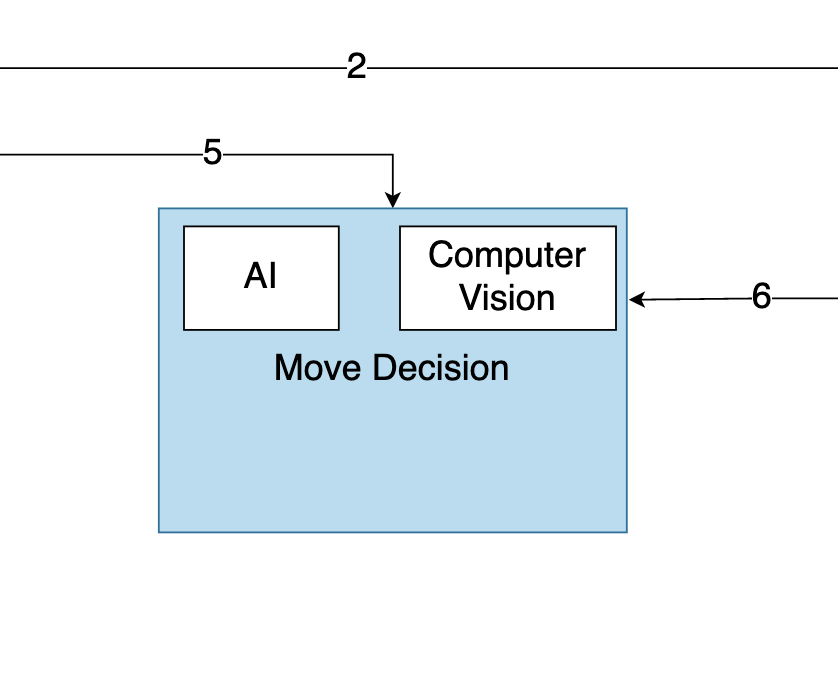
\includegraphics[width=0.60\textwidth]{images/move_decision.png}
 \caption{Example subsystem description diagram}
\end{figure}

\subsubsection{Subsystem Hardware}
%A description of any involved hardware components for the subsystem.
This subsystem requires the computer to utilize artificial intelligence aspect of the decision making.

\subsubsection{Subsystem Operating System}
%A description of any operating systems required by the subsystem.
The subsystem requires Linux distribution Ubuntu 22.04 LTS.

\subsubsection{Subsystem Software Dependencies}
%A description of any software dependencies (libraries, frameworks, design software for mechanical parts or circuits, etc) required by the subsystem.
The subsystem will use python libraries designed for artificial intelligence.

\subsubsection{Subsystem Programming Languages}
%A description of any programming languages used by the subsystem.
This subsystem will use the Python 3.10.6 programming language.

\subsubsection{Subsystem Data Structures}
%A description of any classes or other data structures that are worth discussing for the subsystem. For example, data being transmitted from a microcontroller to a PC via USB should be first be assembled into packets. What is the structure of the packets?
N/A

\subsubsection{Subsystem Data Processing}
%A description of any algorithms or processing strategies that are worth discussing for the subsystem. If you are implementing a well-known algorithm, list it. If it is something unique to this project, discuss it in greater detail.
N/A

\subsection{Computer Vision}
%Descibe at a high level the purpose and basic design of this subsystem. Is it a piece of hardware, a class, a web service, or something else? Note that each of the subsystem items below are meant to be specific to that subystem and not a repeat of anything discussed above for the overall layer.
The Computer Vision interacts with the frames received from the camera to determine the player's move.

% \begin{figure}[h!]
% 	\centering
%  	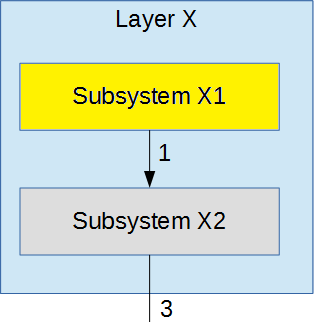
\includegraphics[width=0.60\textwidth]{images/subsystem}
%  \caption{Example subsystem description diagram}
% \end{figure}

\subsubsection{Subsystem Hardware}
%A description of any involved hardware components for the subsystem.
The subsystem will be using a camera to receive frames of the checkers position for both the players and will also use the computer for the computer vision process.

\subsubsection{Subsystem Operating System}
%A description of any operating systems required by the subsystem.
N/A

\subsubsection{Subsystem Software Dependencies}
%A description of any software dependencies (libraries, frameworks, design software for mechanical parts or circuits, etc) required by the subsystem.
This subsystem will use OpenCV and NumPy for the software dependencies.

\subsubsection{Subsystem Programming Languages}
%A description of any programming languages used by the subsystem.
This subsystem will use the Python 3.10.6 programming language.

\subsubsection{Subsystem Data Structures}
%A description of any classes or other data structures that are worth discussing for the subsystem. For example, data being transmitted from a microcontroller to a PC via USB should be first be assembled into packets. What is the structure of the packets?
N/A

\subsubsection{Subsystem Data Processing}
%A description of any algorithms or processing strategies that are worth discussing for the subsystem. If you are implementing a well-known algorithm, list it. If it is something unique to this project, discuss it in greater detail.
N/A



